\documentclass[../Thesis_AHoecherl.tex]{subfiles}

\begin{document}

    In this chapter the results produced for the thesis are presented. We will first show with a small sample portfolio that numerical Euler allocation of \gls{SA-CCR} is possible in section \ref{sec:Exemplary Euler allocation of SA-CCR under consideration of margining}. On these exemplary portfolios we will also point out a couple of observations highlighting how an Euler allocation can offer great insight due to its risk sensitive nature.

    Afterwards, section \ref{sec:Consideration of edge cases} lists scenarios, under which Euler allocation prerequisites are violated and suggests approaches on how to mitigate these issues or proposes a workaround.

    \section{Exemplary Euler allocation of SA-CCR under consideration of margining\label{sec:Exemplary Euler allocation of SA-CCR under consideration of margining}}

    In this section we assume, that the minimum transfer amount, variation margin threshold and initial margin threshold as defined in section \ref{Margining} are all zero. This means, that the margin calculated by the used variation margin and initial margin model is entirely incorporated in the \gls{SA-CCR} model for \gls{EAD} calculation.

    The reason for this is, that assumptions other than zero for the thresholds and \gls{MTA} generally violate the homogeneity prerequisite for Euler allocation. In practice, this is a strong and somewhat unrealistic assumption as for example an initial margin threshold of 50Mn is usual for bilateral portfolios as it is the highest amount allowed by the regulator \cite[Requirement 2.2]{BCBS_MarginRequirements}. Due to the high practical relevance, the impact of thresholds and \gls{MTA} on Euler allocation is analyzed in detail in section \ref{sec:Consideration of edge cases}.   

    \subsection{Exemplary allocation of SA-CCR for a small portfolio of equity options\label{sec:Exemplary allocation of SA-CCR for a small portoflio of equity options}}

    % \todo{Ensure that there are no issues with the currencies. EAD should actually be EUR and needs to be converted to USD}

    In this section we analyze an Euler allocation of a small portfolio of equity options. The detailed computation steps are demonstrated in appendix \ref{sa-ccr-euler-allocation-of-an-exemplary-equity-portfolio}. 
    First, we consider a portfolio consisting of two million call options and three million put option on Adidas. All options are struck at the current stock price and long. Obviously, the two positions are in a hedge relation and being at the money long options, both positions do have a significant, positive present value. 
    
    With the \gls{ISDA SIMM} and \gls{SA-CCR} portfolio risk measures as introduced in sections \ref{sec:The ISDA-SIMM model} and \ref{SA-CCR} and considering different margining approaches we can calculate portfolio risk measure values displayed the portfolio risk measure column of table \ref{tab:2TradeEquityResults}.
    % Table generated by Excel2LaTeX from sheet 'Sheet1'
    \begin{table}[htbp]
        \centering
        \begin{tabular}{l||r|r|r}
            & Portfolio Risk Measure & \makecell{Allocation to \\ 2Mn ADS Call} & \makecell{Allocation to \\ 3Mn ADS Put} \\
                \toprule
        SIMM  & 14,231,564 EUR & -33.75\% & 133.75\%  \\
        \gls{EAD} No margin & 37,643,536 EUR & 99.21\% & 0.79\%  \\
        \gls{EAD} \gls{VM} only & 3,519,458 EUR & 232.47\% & -132.47\%  \\
        \gls{EAD} \gls{VM} and \gls{IM} & 345,874 USD  & 622.10\% & -522.10\% \\
        \end{tabular}%
        \caption{Risk measure results for exemplary equity portfolio}
        \label{tab:2TradeEquityResults}%
    \end{table}%
    It can be seen that incorporation of the variation margin significantly drops the portfolio EAD. The main reason for this is that the RC in formula \ref{eq:SA-CCR EAD} drops from 18.5Mn which is equal to the portfolio \gls{PV} to zero when \gls{VM} is incorporated.
    The additional overcollateralization of 14.2Mn USD through \gls{IM} is then the reason for the \gls{EAD} to again drop by 90\% to 346k USD when \gls{IM} is incorporated in addition to \gls{VM}.

    We can now calculate the Euler allocation by applying the forward difference formula \ref{eq:forward difference} with a bump size of $\epsilon = 0.0001$ as this is the first time this is explicitly done we are writing this down step by step for \gls{EAD} under consideration of \gls{VM} and IM.

    \begin{enumerate}
        \item We increase the position in Adidas call options by $\epsilon$ adding 200 call options to the portfolio.
        \item We recalculate the \gls{EAD} of the updated portfolio as $\rho_{\text{Inc Call}}$ and remove the 200 Mn call options again.
        \item We repeat this with a position increase of 100 Adidas put options yielding result $\rho_{\text{Inc Put}}$.
        \item We now use the \emph{bumped} risk measure results and the original $\rho$ of 345,874 USD as displayed in table \ref{tab:2TradeEquityResults} to yield the allocation.
        \item The allocated value for the call position is $\text{alloc}_\text{call}=\frac{\rho{\text{Inc Call}-\rho}}{0.0001} = 2.152 \text{ Mn USD}$.
        \item The allocated value for the put position is $\text{alloc}_\text{call}=\frac{\rho{\text{Inc Put}-\rho}}{0.0001} = -1.806 \text{ Mn USD}$.
        \item This yield the relative allocated values of 622\% and -522\% displayed in table \ref{tab:2TradeEquityResults}.
    \end{enumerate}

    Comparing the allocations of the different risk measures in table \ref{tab:2TradeEquityResults} with each other uncovers a couple of interesting observations. 
    
    First, under consideration of no margin, the contribution of the put position is close to zero. 
    The reason for this is that a marginal increase in the put position impacts the PFE and RC component of equation \ref{eq:SA-CCR EAD} differently. A marginal notional increase increases the RC due to associated increasing positive market value.
    The potential future exposure (PFE) on the other hand decreases, since the put hedges some of the portfolio risk incurred by the larger call position.

    Secondly, for the \gls{ISDA SIMM} risk measure the call position is considered as a hedge position, i.e. has a negative allocated value, while for the \gls{VM} only \gls{EAD} model the put position is considered a hedge. 
    A marginal increase in the call position decreases the charged \gls{IM} while it increases the calculated \gls{EAD} under consideration of \gls{VM} only. 
    These two effects reinforce each other when allocating the \gls{EAD} under consideration of \gls{VM} and IM. Here, a marginal increase in the call position simultaneously increases the portfolio risk under the \gls{SA-CCR} \gls{EAD} risk measure while also resulting in a decrease in received \gls{IM} and therefore reducing overcollateralization which further raises the calculated EAD. 
    
    On the other hand, a marginal increase in the put position decreases the \gls{EAD} risk measure while simultaneously increasing overcollateralization. This is the reason for the stark increase of the relative allocated risk from the \gls{VM} only case to the \gls{VM}+IM case.

    Finally, it is worth discussing why the \gls{ISDA SIMM} risk measure and the \gls{SA-CCR} risk measure evaluate the portfolio so differently with one considering the put a hedge position while the other one considers the call as the hedge position.
    Due to the large differences between the two models and the dependency of the \gls{ISDA SIMM} model on market data is is difficult to pinpoint a single driving factor for this phenomenon.
    However, the different holding periods of ten days for the \gls{ISDA SIMM} model and one year for the \gls{SA-CCR} model appears to be a likely candidate. Indeed, if we reduce the maturity of the options from one year to ten days and thereby effectively reduce the holding period of the \gls{SA-CCR} model to ten days we can see from the results in table \ref{tab:2TradeEquity10dayEAD} that the \gls{SA-CCR} model then considers the smaller call position to be the hedge trade.

    % Table generated by Excel2LaTeX from sheet 'Sheet1'
    \begin{table}[htbp]
        \centering
        \begin{tabular}{l||r|r|r}
                & \makecell{Allocation to \\ 2Mn ADS Call 10D} & \makecell{Allocation to \\ 3Mn ADS Put 10D} & Portfolio Risk Measure \\
                \toprule
                \gls{EAD} \gls{VM} only & -358.06\% & 458.06\% & 1,701,707 EUR \\
        \end{tabular}%
        \caption{Allocation amount under ten day maturity}
        \label{tab:2TradeEquity10dayEAD}%
    \end{table}%

    A reliable test, whether the Euler allocation was successful and therefore if the allocated function exhibits homogeneity is to calculate if equation \ref{eq:Euler theorem of positive homogeneous functions} holds.

    When doing so the value allocated to a certain trade $\text{alloc}_{t}$ is $\frac{\partial f}{\partial x_i}$ and the portfolio risk measure $\rho$ is the $f(x)$. The degree $k$ is one. 
    This results in formula \ref{eq:allocation_homogeneity_test} which is just an alternative notation of Eulers theorem of homogeneous functions. If this equation is met, the risk measure $\rho$ does locally exhibit homogeneity and the results $\text{alloc}_t$ can be considered a risk sensitive allocation and used for risk analysis or portfolio optimization purposes.

    \begin{align}
        \label{eq:allocation_homogeneity_test}
        \sum_t{\text{alloc}_t} = \rho
    \end{align}
    
    
    For the allocation of \gls{EAD} under \gls{VM} and \gls{IM} shown in table \ref{tab:2TradeEquityResults} equation \ref{eq:allocation_homogeneity_test} does not hold as we yield a residual of 1068 EUR or about 0.3\% of the portfolio risk measure. Since $\text{alloc}_t$ has just been approximated with a finite difference some deviation may be expected. This deviation appears to be within the expected order of magnitude of a forward difference approximation of the two derivatives.

    The approximated derivate for the call position is $6.221 * 345,874 = 2.151 \text{Mn}$ while the approximated derivative of the put position is $-1.806 \text{Mn}$. 
    In absolute terms this results in a sum of about 4Mn. Considering the $\epsilon = 0.0001$ this indicates, that the sum of the error of the two derivatives should be in the order of $\mathcal{O}\left(4\text{Mn}/0.0001 = 400 \text{USD}\right)$ which is in line with the observed deviation.

    Theoretically, application of a central difference approach should bring the order of magnitude of the error down to $\mathcal{O}\left(4Mn/0.0001^2 = 0.04 \text{USD}\right)$.
     This behavior can also be observed. 
    If the partial derivatives are instead calculated as $(\rho_{Incr}-\rho_{Decr})/0.0001$ the sum of the allocations deviates from the portfolio risk measures by only 0.01 EUR. 
    This indicates that for proper native additivity of the Euler allocation of EAD, the computationally more expensive central difference approach should be used.
    An even stronger case for application of a central difference approach will be made in section \ref{sec:Allocation of hedged portfolios}.

    \subsection{Exemplary allocation of SA-CCR for a small portfolio of interest rate derivatives\label{sec:Exemplary allocation of SA-CCR for a small portfolio of interst rate derivatives}}

    In this section we investigate a small rates portfolio. This section will further highlight how the interaction of the two \gls{EAD} and initial margin risk measures can yield surprising results stressing the need for a risk sensitive allocation methodology for analysis purposes. The detailed computation steps are demonstrated in appendix \ref{euler-allocation-of-an-exemplary-rates-portfolio}.

    Initially, we consider a 1Bn USD Receiver \gls{IRS} and a 180Mn EUR Payer \gls{IRS} and create three portfolios. The first only contains the USD \gls{IRS}, the second only contains the EUR \gls{IRS} and the third contains both trades.
    For these portfolios we calculate three risk measures: the \gls{ISDA SIMM} initial margin, the \gls{EAD} under consideration of \gls{VM} and the \gls{EAD} under consideration of \gls{VM} and IM. The results are displayed in table \ref{tab:2TradeRatesResults}.

    \begin{table}[htbp]
        \centering
        \begin{tabular}{l||r|r|r}
                & \gls{EAD} \gls{VM} only &\gls{ISDA SIMM} & \gls{EAD} \gls{VM} + \gls{IM} \\
                \toprule
        EUR Swap & 1,957,315 USD & 6,079,460 USD & 286,420 USD \\
        USD Swap & 10,873,970 USD & 28,762,683 USD & 2,014,873 USD \\
        Both Swaps & 12,831,284 USD & 28,059,093 USD & 3,074,959 USD \\
        \end{tabular}%
        \caption{Risk measures for exemplary rates portfolio}
        \label{tab:2TradeRatesResults}%
    \end{table}%

    Interest rate risks across different currencies are handled differently between the \gls{SA-CCR} and the \gls{ISDA SIMM} model.
    In the \gls{SA-CCR} model each interest rate currency forms a separate so called \emph{hedging set}. \gls{SA-CCR} does not allow for any hedge effects across the borders of a hedging set.
    We can observe this in the 'EAD \gls{VM} only' column of table \ref{tab:2TradeRatesResults}, since the \gls{EAD} of the portfolio containing both trades is simply the sum of the two standalone portfolios.
    The \gls{ISDA SIMM} risk measure on the other hand does allow hedge effects across currencies within the interest rate asset class. When aggregating sensitivities across multiple currency buckets, \gls{ISDA SIMM} assumes a correlation of 22\% \cite[Section D.2]{SIMM}.
    This does show in the \gls{ISDA SIMM} column of table \ref{tab:2TradeRatesResults} with the \gls{ISDA SIMM} charged for the portfolio containing both trades being smaller than the sum of the two standalone portfolios.
    
    This difference in models leads to the phenomenon that can be observed in the \gls{EAD} under \gls{VM} and \gls{IM} column. The calculated \gls{EAD} for the portfolio of both \gls{IRS} is significantly higher than the sum of the \gls{EAD} of the two standalone portfolios.
    We have found a counterexample showing that \gls{SA-CCR} under consideration of \gls{VM} and \gls{IM} is not a sub-additive risk measure.
    Subadditivity is one of the properties of a coherent risk measure and counterexamples showing that a risk measure does not exhibit subadditivity can for example be constructed for all \gls{VaR}-based risk measures. However, for \gls{EAD} under \gls{IM} and \gls{VM} it appears to be especially simple to construct a counterexample.

    The \gls{SA-CCR} model considers the portfolio of both trades to be just as risky as the two trades independently. However, the available overcollateralization of the portfolio with both trades is relatively lower than the overcollateralization of the two standalone portfolios since the \gls{ISDA SIMM} model does recognize hedge effect trades. This constellation leads to the observed effect that the \gls{EAD} of the joint portfolio is higher than the sum of the standalone \gls{EAD} of the trades.

    When performing an Euler allocation of the different risk measures of the portfolio containing both \gls{IRS} we yield the allocation as depicted in table \ref{tab:2TradeRatesAllocation}.

    \begin{table}[htbp]
        \centering
        \begin{tabular}{l||r|r|r}
                & \makecell{Allocated \\ \gls{EAD} \gls{VM} only} & \makecell{Allocated \\ \gls{ISDA SIMM}} & \makecell{Allocated \\ \gls{EAD} \gls{VM} + IM} \\
                \toprule
        180Mn EUR Swap & 15.25\% & -0.19\% & 34.95\% \\
        1000Mn USD Swap & 84.75\% & 100.19\% & 65.05\% \\
        \end{tabular}%
        \caption{Risk measure allocation of exemplary rates portfolio}
        \label{tab:2TradeRatesAllocation}%
    \end{table}%
    
    The results are related to those observed in table \ref{tab:2TradeEquityResults}. As $15.25\% * 12.83Mn = 1.96Mn$ the Euler allocation results coincide with the standalone results when allocating the \gls{EAD} under consideration of \gls{VM} only. 
    For the allocation of \gls{ISDA SIMM} on the other hand the EUR trade is considered a hedge trade and almost none of the risk measure is allocated to it. 
    The fact that the EUR trade reduces overcollateralization then also leads to the overproportionate fraction of the risk measure that is allocated to it under consideration of \gls{VM} and IM.
    
    Considering the larger USD swap as the baseline trade the EUR swap contribution to the portfolio \gls{EAD} under \gls{IM} and \gls{VM} is overproportionate since it is considered to be a risk mitigating trade by the \gls{ISDA SIMM} model while the \gls{SA-CCR} model considers it to increase the risk. The opposite phenomenon can be observed when we add a USD receiver swaption as a third trade to the portfolio.

    For this we add a one year swaption on a five year 500Mn USD receiver swap to the portfolio. The risk measures of the resulting portfolio are allocated and the result displayed in table \ref{tab:3TradeRatesAllocation}. 

    \begin{table}[htbp]
        \centering
        \begin{tabular}{l||r|r|r}
                & \makecell{Allocated \\ \gls{EAD} \gls{VM} only} &\makecell{Allocated \\ \gls{ISDA SIMM}} &\makecell{Allocated \\ \gls{EAD} \gls{VM} + IM} \\
                \toprule
        180Mn EUR Swap & 17.70\% & 0.50\% & 43.69\% \\
        1000Mn USD Swap & 98.33\% & 80.07\% & 125.93\% \\
        500Mn USD Swaption & -16.04\% & 19.44 \% & -69.62\\
        \end{tabular}%
        \caption{Allocation results after addition of a swaption}
        \label{tab:3TradeRatesAllocation}%
    \end{table}%
    As can be seen, the swaption is considered to be marginally risk decreasing by the \gls{EAD} risk measure with only \gls{VM} while it is considered to be a risk increasing trade by the \gls{ISDA SIMM} risk measure. Consequently, the swaption reduces the \gls{EAD} under consideration of \gls{VM} and \gls{IM} by an overproportionate amount as it decreases risk while increasing overcollateralization which is indicated by the large negative Euler allocation.

    In line with the results of the Euler allocation we can see in table \ref{tab:3TradeRatesResults} that inclusion of the swaption increases portfolio \gls{ISDA SIMM} by 24\%, while decreasing portfolio \gls{EAD} under \gls{VM} by -14\% and portfolio \gls{EAD} und \gls{VM} and \gls{IM} by -48\%. This is exactly the opposite effect as observed for the EUR swap beforehand.

    \begin{table}[htbp]
        \centering
        \begin{tabular}{l||r|r|r}
                & \gls{EAD} \gls{VM} only &\gls{ISDA SIMM} & \gls{EAD} \gls{VM} + \gls{IM} \\
                \toprule
        Portfolio & 11,058,114 USD & 34,796,088 USD & 1,586,748 USD \\
        \end{tabular}%
        \caption{Impact of the swaption on the portfolio risk measure}
        \label{tab:3TradeRatesResults}%
    \end{table}%

    For the swaption it is more difficult to pinpoint where the difference between the \gls{ISDA SIMM} and \gls{SA-CCR} model that results in the very different risk assessment of the swaption in relation to the rest of the portfolio is originating.
    Sensitivities of the swaps and swaption are calculated very differently between the two models with the \gls{ISDA SIMM} model being based on current market data whilst the \gls{SA-CCR} makes much more simplifying assumptions. 

    \subsection{Exemplary allocation of SA-CCR on subportfolios\label{sec:Exemplary allocation of SA-CCR on subportfolios}}

    One of the advantages of the Euler allocation is, that once allocated, values on trade level can be aggregated to also produce risk sensitive results for subportfolios. It is also possible to directly allocate risk metrics on subportfolios if no further granularity is required and thereby saving computation time. The detailed computation steps for the results of this section are demonstrated in appendix \ref{sa-ccr-euler-allocation-of-an-exemplary-multi-asset-class-portfolio}. 

    For this we put the five exemplary derivatives of the two previous sections in a joint portfolio, i.e. the EUR \gls{IRS}, the USD \gls{IRS}, the USD swaption and the position in Adidas put and call options.
    The resulting portfolio risk measures are displayed in the last row of table \ref{tab:multiAssetResult} with the portfolio results of the standalone portfolios from the previous section displayed as reference.

    \begin{table}[htbp]
        \centering
        \begin{tabular}{l||r|r|r}
                & \gls{EAD} \gls{VM} only &\gls{ISDA SIMM} & \gls{EAD} \gls{VM} + \gls{IM} \\
                \toprule
        Equity Portfolio & 3,519,458 USD & 14,231,564 USD & 345,874 USD \\
        Rates Portfolio & 11,058,114 USD & 34,796,088 USD & 1,586,748 USD \\
        \midrule
        Equity \& Rates Portfolio & 14,577,571 USD & 49,027,652  USD & 1,890,742 USD \\
        \end{tabular}%
        \caption{Risk measure results of a mixed equity and rates portfolio}
        \label{tab:multiAssetResult}%
    \end{table}%

    As we can see, for \gls{EAD} under \gls{VM} and \gls{ISDA SIMM} the multi asset class portfolio is simply the sum of the risk measures of the portfolios containing only trades of the individual asset class.
    The reason for this is, that for both models, \gls{SA-CCR} and \gls{ISDA SIMM} no hedge effects are recognized between different asset classes.
    Nevertheless, for \gls{EAD} under \gls{VM} and \gls{IM} we can observe in table \ref{tab:multiAssetResult} that the \gls{EAD} of the multi asset class portfolio is slightly lower than the sum of the equity and the rates portfolio. 
    The reason for this is that initial margin pledged for interest rates trades may also be used to mitigate losses caused by equity trades and vice versa. This slightly increases the overcollateralization of the joint portfolio leading to a lower \gls{EAD} under \gls{VM} and IM.

    When allocating the joint portfolio risk measure to the individual trades we yield the trade allocations displayed in table \ref{tab:multiAssetAllocation} and can also aggregate the results on subportfolio level as shown in the table for an equity and rates subportfolio.

    \begin{table}[htbp]
        \centering
        \begin{tabular}{l||r|r|r}
                & \makecell{Allocated \\ \gls{EAD} \gls{VM} only} &\makecell{Allocated \\ \gls{ISDA SIMM}} & \makecell{Allocated \\\gls{EAD} \gls{VM} + \gls{IM}} \\
                \toprule
        2Mn ADS Call & 8,181,543 USD & -4,802,460 USD & 2,959,180 USD \\
        3Mn ADS Put & -4,662,085 USD & 19,034,023 USD & -2,643,342 USD \\
        \midrule
        Equity subportfolio & 3,519,458 USD & 14,231,564 USD & 315,837 USD \\
        \toprule
        180Mn EUR Swap & 1,957,315 USD & 172,265 USD & 630,350 USD \\
        1000Mn USD Swap & 10,873,970 USD & 27,859,887 USD & 1,921,998 USD \\
        500Mn USD Swaption & -1,773,170 USD & 6,763,936 USD & -977,443 USD \\
        \midrule
        Rates subportfolio & 11,058,114 USD & 34,796,088 USD & 1,574,905 USD \\
        \end{tabular}%
        \caption{Allocation result of the mixed portfolio}
        \label{tab:multiAssetAllocation}%
    \end{table}%

    If an allocation on trade level is more granular than necessary it is also possible to directly allocate the portfolio risk measure on subportfolios. Therefore, each $u_i$ from equation \ref{eq: u formula} needs to be interpreted not as a single trade but rather as a selection of trades.
    When calculating the Euler allocation with a central difference approach this means that the notional of all trades within the subportfolio is bumped simultaneously by a relative amount $\epsilon / 2$.
    This does save computation time as in the example shown in table \ref{tab:multiAssetAllocation} only four new portfolio risk measure aggregations are necessary to allocate to the equity and rates subportfolio directly while ten aggregations are necessary to allocate a risk measure on all of the five trades. An allocation of the subportfolios is calculated with this approach in appendix \ref{sa-ccr-euler-allocation-of-an-exemplary-multi-asset-class-portfolio} and yields exactly the same result as the summed up subportfolio results in table \ref{tab:multiAssetAllocation}.

    This might also be a valid approach for a risk analysis architecture that calculates allocations only when requested by a user in real time on the required aggregation level. 

    % Figure \ref{fig:C for ITM IRS} also showcases the trivial result that the Variation Margin is a homogeneous function - the value of the trade scales linearly with the notional.
    
    % Critically, this result can also be transferred to any SA-CCR allocation approach that would treat C as an externally given constant value as locally, treating C as a constant value is the same as consideration of a \gls{MTA}. 
    % In both cases the slope of C is zero. 

    \section{Consideration of edge cases\label{sec:Consideration of edge cases}}

    While numerical Euler allocation of \gls{SA-CCR} and \gls{ISDA SIMM} is generally possible as shown in section \ref{sec:Exemplary Euler allocation of SA-CCR under consideration of margining}, a couple of cases can be identified, in which Euler allocation fails since its prerequisites of homogeneity and differentiability are violated.
    Both, \gls{ISDA SIMM} and \gls{SA-CCR} are complex, convoluted formulas, making general observations on differentiability and homogeneity difficult.
    In fact, we will see that depending on the portfolio and parametrization of the collateral agreement, both \gls{ISDA SIMM} and \gls{SA-CCR} are not homogeneous risk measures, and that they are both occasionally not partially differentiable w.r.t. position size.
    
    In this section, all identified cases under which prerequisites for Euler allocation are violated are presented and for some a workaround is presented to allow nevertheless for risk sensitive and naturally additive allocation.
    
    \subsection{Allocation when an ISDA SIMM liquidity threshold is exceeded\label{sec:Allocation when an ISDA-SIMM liquidity threshold is exceeded}}
    
    As pointed out in section \ref{sec:Euler allocation} a risk measure needs to exhibit positive homogeneity of degree 1 to be able to perform an Euler allocation.
    This precondition is violated if a liquidity threshold of the \gls{ISDA SIMM} model is exceeded.

    We can show this by exploring whether \gls{ISDA SIMM} does exhibit positive homogeneity for a minimal example.
    
    For this we set up an USD Libor \gls{IRS} with ten years time to maturity and a notional of 200 billion USD. This is our initial portfolio $\mathbf{u}$. \gls{ISDA SIMM} would fulfill the required positive homogeneity condition if $a \rho(\mathbf{u}) = \rho(a \mathbf{u})$ for $a>0$. In figure \ref{fig:homogeneity of ISDA SIMM} $\rho(a\mathbf{u})$ is plotted for $0<a\leq 2$ in blue. 
    \begin{figure}
        \centering
        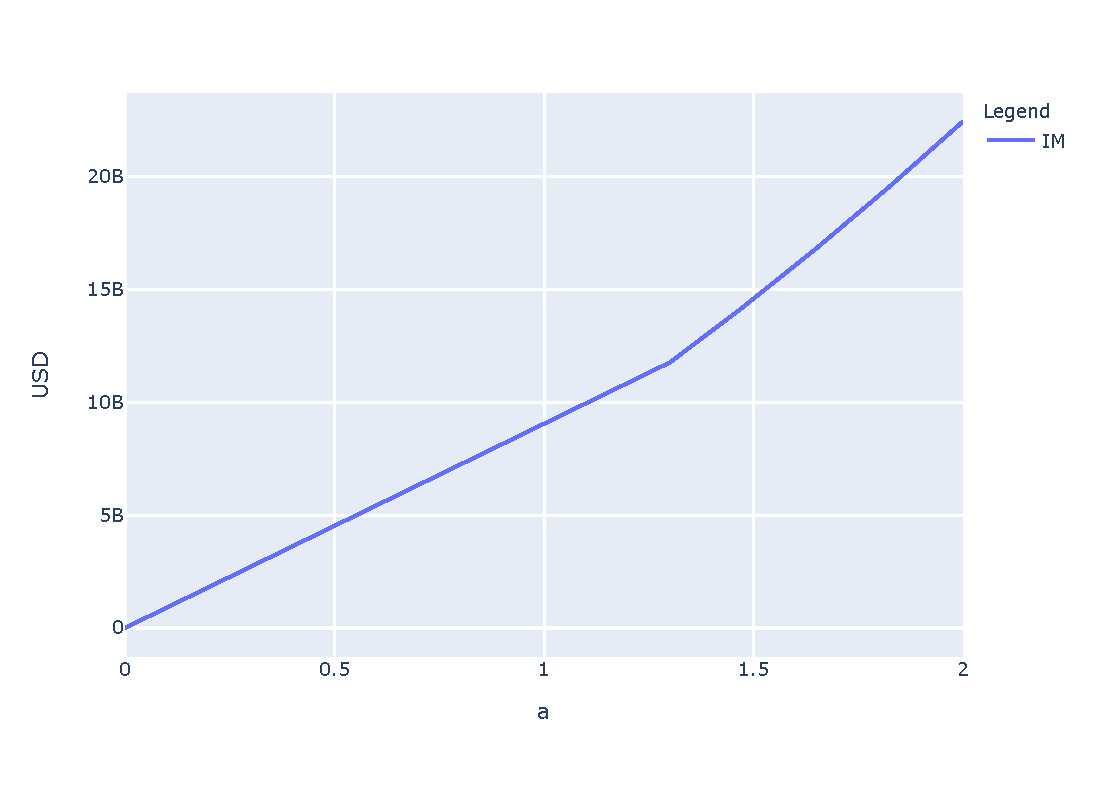
\includegraphics{Graphics/ISDA_SIMM_homogenity.pdf}
        \caption[Homogeneity of ISDA SIMM]{ISDA SIMM calculated for different notionals invested in the trade with $a=1$ being an investment of 200 billion USD}
        \label{fig:homogeneity of ISDA SIMM}
    \end{figure}
    The function exhibits homogeneity for $0<a<1.3$ but not for higher $a$. 
    The reason for this is, that at this point the concentration risk charge of \gls{ISDA SIMM} does kick in.
    The concentration risk for interest rate risks for our minimal example is defined as \cite[Article 7.b]{SIMM}
    \begin{align*}
        CR = \max\left(1,\left(\frac{\lvert\sum{s}\rvert}{T}\right)^{1/2}\right)
    \end{align*}
    with $s$ being the sensitivities against USD interest rate risk and T being 230Mn USD as specified in \cite[Article 74]{SIMM}. Due to subsequent variance-covariance aggregation the concentration risk impacts the calculated \gls{IM} as
    \begin{align*}
        IM_{\text{with conc. risk}} = CR^2 \cdot IM_{\text{without conc. risk}}
    \end{align*}
    This causes the change in slope and implied loss of homogeneity visible in figure \ref{fig:homogeneity of ISDA SIMM}. If the portfolio would consist of a more diverse set of risk factors than the minimal example displayed in figure \ref{fig:homogeneity of ISDA SIMM} the associated concentration risk would kick in at different levels of $a$.
    The slope of the function would increase with each additional concentration risk not being floored at one any more. 
    
    It is important to note that as soon as the sensitivity against a single risk factor in the portfolio is above the concentration threshold the \gls{ISDA SIMM} risk measure does not exhibit homogeneity anymore.
    
    Even a trivial example with just one trade is sufficient to show that Euler allocation does not work in the inhomogeneous part of the \gls{ISDA SIMM} equation.
    For this, we compare two sample portfolios one consisting of one USD \gls{IRS} with 200 bn notional and one consisting of one USD \gls{IRS} with 400 bn notional.
    Critically, the second portfolio is penalized by the model since its USD \gls{IRS} risk is too large. We calculate the Euler calculation with a forward finite difference approach as displayed in equation \ref{eq:forward difference}.
    
    Assuming that we calculate the finite difference with an $\epsilon = 0.0001$ this means that we calculate the \gls{ISDA SIMM} of an \gls{IRS} with 200Bn notional ($SIMM_{200Bn}$) and the \gls{ISDA SIMM} of an equivalent \gls{IRS} with 200.02 Bn notional ($SIMM_{200.02Bn}$) and this yields an Euler allocation to this trade as
    \begin{align*}
        \frac{SIMM_{200.02Bn} - SIMM_{200Bn}}{0.0001} = 9.04Bn
    \end{align*}
    We can see in figure \ref{fig:homogeneity of ISDA SIMM} that this value is both, the slope and the \gls{IM} value at $a = 1$. The portfolios \gls{IM} was correctly fully allocated to the single trade of which it consists. 
    
    However, performing the same calculation for an equivalent \gls{IRS} with 400Bn notional yields
    \begin{align*}
        \frac{SIMM_{400.04Bn} - SIMM_{400Bn}}{0.0001} = 33.67Bn
    \end{align*}
    again, we can refer to figure \ref{fig:homogeneity of ISDA SIMM} to check if this is a reasonable allocation result. As $a=1$ represents the \gls{IM} charge for investing 200Bn of notional in the \gls{IRS}, $a=2$ represents an investment of 400Bn notional. The associated \gls{IM} is just 22.44Bn - allocating 33.67Bn of the risk measure to the only trade in the portfolio is therefore clearly wrong. The Euler allocation of 33.67Bn can also be read off figure \ref{fig:homogeneity of ISDA SIMM} - it is the slope at $a=2$ times two.

    This result extends to the Euler allocation of the \gls{SA-CCR}. When allocation of the \gls{IM} is not possible any more, allocation of the \gls{SA-CCR} is neither if initial margin is taken into consideration during \gls{SA-CCR} calculation.

    % Euler allocation of SA-CCR also does not work if the calculated C does not exhibit homogeneity, i.e. if a concentration risk threshold of the ISDA-SIMM model is exceeded. Again using the 400Bn IRS from \ref{Allocation of initial margin} we calculate an EAD\textsubscript{400Bn IRS} of 843.5Mn but, despite not applying an MTA, Euler allocation yields a vastly different amount of $ \frac{\text{EAD\textsubscript{200.02Bn IRS}}-\text{EAD\textsubscript{200Bn IRS}}}{0.0001} = 201.0Mn $. If for a given portfolio C does not exhibit homogeneity, neither does SA-CCR and therefore Euler allocation of SA-CCR is not possible for such portfolios. \todo{Paragraph needs to be tidied up as it has been relocated}
    
    % As can already seen by the notional of the exemplary trade, the liquidity thresholds imposed by ISDA-SIMM are relatively high and will not be exceeded by the majority of bilateral portfolios.
    
    % \todo{Insert explanation that this can't really be fixed.}

    \subsection{Incorporation of a minimum transfer amount and threshold}\label{sec:Incorporation of a minimum transfer amount and threshold}

    To allocate \gls{SA-CCR} under consideration of margining, the available collateral $C$ is of special interest. As pointed out in table \ref{tab:Margin in SA-CCR} depending on the margining approach, C can be calculated as $C = \text{VM}$ or $C = \text{VM} + \text{IM}_{\text{received}}$. 
    
    The actually exchanged collateral, however has to be calculated under consideration of the threshold and minimum transfer amount as displayed in equation \ref{eq:C}. With this consideration of threshold and minimum transfer amount $C$ is not a homogeneous function. 

    \begin{figure}
        \centering
        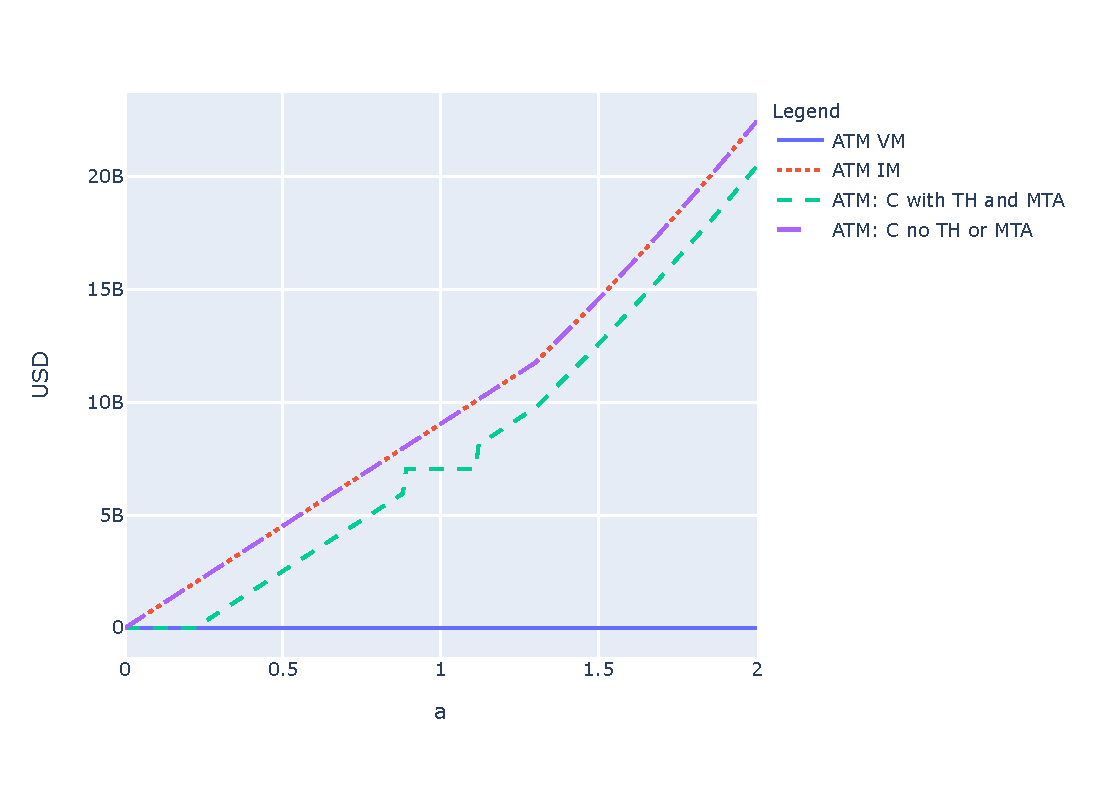
\includegraphics{Graphics/C_and_its_components_for_ATM_IRS.pdf}
        \caption[Homogeneity of \gls{SA-CCR} for an at the money \gls{IRS}]{VM, IM, C and C under consideration of \gls{TH} and \gls{MTA} for a portfolio consisting of a single at the money interest rate swap. Values are calculated based on different notionals invested in the \gls{IRS} with $a=1$ referring to a notional of 200Bn USD. More details on creation can be found in Appendix \ref{homogeneity-of-c-for-a-single-trade-portfolio}.}
        \label{fig:C for ATM IRS}
    \end{figure}

    \begin{figure}
        \centering
        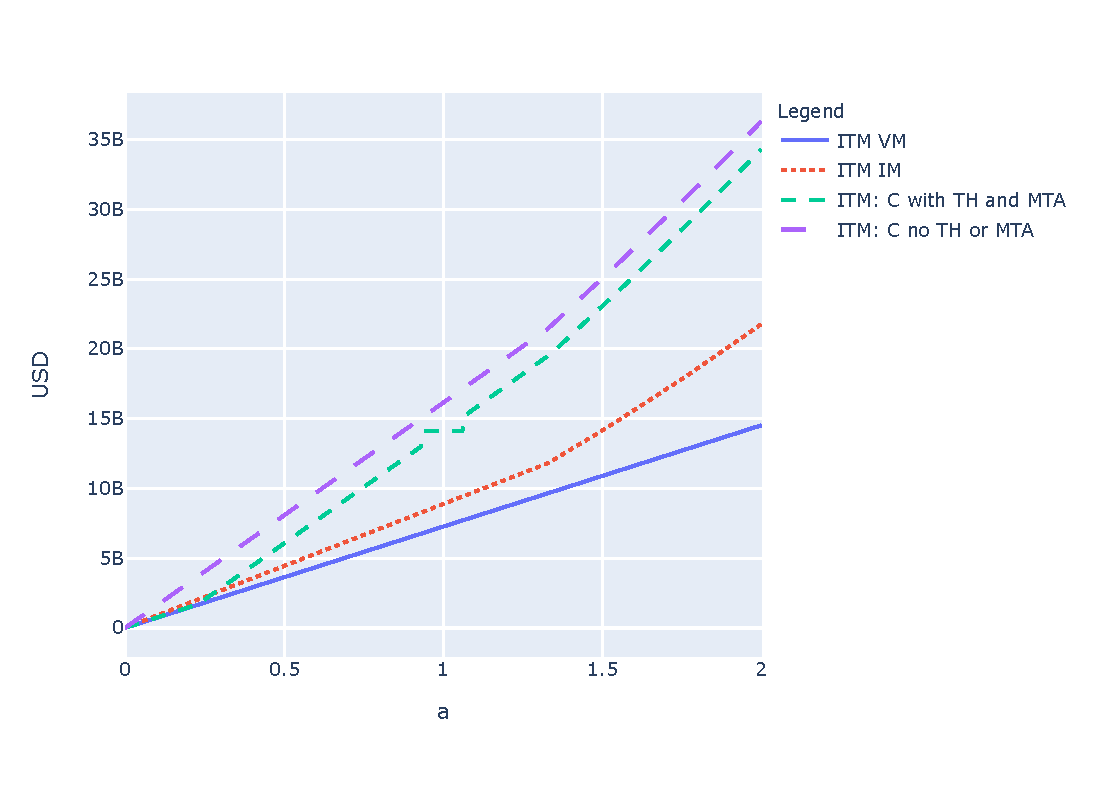
\includegraphics{Graphics/C_and_its_components_for_ITM_IRS.pdf}
        \caption[Homogeneity of \gls{SA-CCR} for an in the money \gls{IRS}]{Same as figure \ref{fig:C for ATM IRS} but for an in the money trade with an payer interest rate at 2\% which is below par.}
        \label{fig:C for ITM IRS}
    \end{figure}
    
    This can exemplary seen in figures \ref{fig:C for ATM IRS} and \ref{fig:C for ITM IRS}. These figures display $C$ for an at the money 10Y USD interest swap and the same swap with a lower fixed rate making it an in the money swap. Again, a very high notional of 200 Bn is chosen to showcase the concentration risk charge of \gls{ISDA SIMM} and the threshold and minimum transfer amount have also been chosen to be very high at 2Bn and 1Bn USD.

    \subsubsection{Incorporation of a VM threshold\label{sec:Incorporation of a VM threshold}}
    
    Generally, a variation margin threshold can not be in place when bilateral initial margin is being exchanged. The reason for this is, that the regulator poses a \gls{VM} threshold of zero as a prerequisite for bilateral initial margining \cite[Requirement 2.1]{BCBS_MarginRequirements}.

    No exchange of \gls{IM} implies that no overcollateralization can be available and therefore margining has no impact on the $PFE$ as defined in formula \ref{eq:PFE}. Instead the \gls{VM} threshold solely impacts the $RC$ which, based on formula \ref{eq:RC}, under \gls{VM} but in absence of \gls{IM} simplifies to $RC = \text{VM Threshold}$ independent of the portfolio constellation. 
    Consequently, a \gls{VM} threshold will always increase the portfolio \gls{EAD} by $1.4*\text{VM threshold}$. Even if the portfolio is empty, the \gls{EAD} will be $1.4 * \text{VM threshold}$.

    When performing an Euler allocation of a portfolio with a \gls{VM} threshold, the sum of the allocations will be $EAD - 1.4 * \text{VM threshold}$. This is arguably a correct result, as this remainder is independent of the trades and even remains when all trades are removed from the portfolio. 
    A bank allocating its \gls{EAD} can decide freely weather the \gls{VM} threshold impact on the \gls{EAD} of $1.4 * \text{VM threshold}$ shall remain unallocated or to allocate it to the trades of the portfolio according to some pro-rata approach.

    Some exemplary calculations exploring the effects of a \gls{VM} threshold can be found in appendix \ref{ead-impact-of-a-variation-margin-threshold}.
    
    \subsubsection{Incorporation of a minimum transfer amount}\label{sec:Incorporation of a minimum transfer amount}

    Again, similar to the exemplary calculation in section \ref{sec:Allocation when an ISDA-SIMM liquidity threshold is exceeded} it can be shown with a trivial example, that Euler allocation of \gls{SA-CCR} is not possible under recognition of a \gls{MTA}. Detailed documentation of this exemplary calculation may be found in appendix \ref{exemplary-sa-ccr-allocation-under-consideration-of-a-minimum-transfer-amount.}.
    
    We consider the same 200Bn \gls{IRS} as in section \ref{sec:Allocation when an ISDA-SIMM liquidity threshold is exceeded}. We assume that the currently posted margin is 9.04Bn which is the calculated \gls{ISDA SIMM} margin. 
    Setting $C$ at 9.04Bn in the \gls{SA-CCR} equation \ref{eq:multiplier} and then calculating the \gls{SA-CCR} \gls{EAD} for this single \gls{IRS} yields an regulatory \gls{EAD} of 582.8Mn USD. Any natively additive allocation should allocate this full amount to the \gls{IRS}.
    The \gls{VM} is zero as the \gls{IRS} is struck at par. 
    \begin{table}[htbp]
        \centering
        \begin{tabular}{c|c|c}
            & $\text{SA-CCR}_{\text{MTA}}$ & $\text{SA-CCR}_{\text{No \gls{MTA}}}$ \\
            \toprule
            Initial C & 9038.2Mn & 9038.2Mn \\
            \midrule
            EAD\textsubscript{200Bn IRS} & 582.8Mn & 582.8Mn \\
            \midrule
            C\textsubscript{200Bn IRS} & 9038.2Mn & 9038.2Mn \\
            \midrule
            C\textsubscript{200.02Bn IRS} & 9038.2Mn & 9039.1Mn \\
            \midrule
            EAD\textsubscript{200.02Bn IRS} & 583.0Mn & 582.9Mn \\
            \midrule
            $\frac{\text{EAD\textsubscript{200.02Bn IRS}}-\text{EAD\textsubscript{200Bn IRS}}}{0.0001}$ & 1425.3Mn & 582.8Mn  \\
        \end{tabular}%
        \caption[Impact of an \gls{MTA} on an allocation]{Numerical Euler allocation of \gls{SA-CCR} with and without consideration of a minimum transfer amount for an example of a portfolio with a single 200Bn notional \gls{IRS}. Euler allocation is only successful if the \gls{MTA} is not considered for the recalculation of the received margin C. A threshold of 0 is assumed.}
        \label{tab:Allocate SA-CCR with MTA calculation}
    \end{table}
    In table \ref{tab:Allocate SA-CCR with MTA calculation} we assume that the initially received collateral is the currently calculated collateral. 
    When calculating the Euler allocation with a forward difference in line with equation \ref{eq:forward difference}, the received collateral when rising the notional to 200.02Bn increases when no \gls{MTA} is assumed while it remains unchanged with consideration of an MTA. 
    Ultimately, this difference leads to a correct allocation of the entire \gls{EAD} to the single \gls{IRS} with the \emph{No MTA} approach while the \emph{MTA} approach obviously yields a wrong result by allocating 244\% of the portfolios \gls{EAD} to its only trade.

    In the above example any adverse impact that the \gls{MTA} may have on the Euler allocation can be mitigated by simply assuming an \gls{MTA} of zero during the calculation of the Euler allocation.
    However, a scenario can be constructed in which this approach still leads to an allocation, whose sum deviates from the portfolio risk measure.

    As established in table \ref{tab:Margin in SA-CCR} the \gls{MTA} impacts the RC of the \gls{SA-CCR} calculation with $RC = \text{TH\textsubscript{IM}} + \text{MTA}$ under \gls{VM} collateralization and $RC = \max{\left(0, \text{MTA} - \text{IM\textsubscript{rec}}\right)}$ under \gls{VM} and \gls{IM} collateralization.
    If only \gls{VM} is exchanged this does not need to be recognized in an Euler allocation. Following the same line of argument that has already been used in section \ref{sec:Incorporation of a VM threshold} the \gls{MTA} increases the \gls{EAD} under all circumstances by a flat amount of $1.4*EAD$ which does not necessarily have to be allocated to any trade.

    On the other hand, if \gls{VM} and \gls{IM} are exchanged a \gls{MTA} does not increase the RC by a flat amount but the impact of the \gls{MTA} on the RC depends on the received initial margin. Accordingly, if $\text{IM\textsubscript{rec}} < MTA$ the impact of a trade on the exchanged initial margin not only impacts the PFE of equation \ref{eq:SA-CCR EAD} but also the RC. This effect is lost if the Euler allocation is calculated under an assumption of $MTA = 0$. An example for this phenomenon is presented in Appendix \ref{impact-of-the-minimum-transfer-amount-on-rc}.

    However, the window for this phenomenon to occur in practice is rather small. If bilateral initial margin is exchanged, the regulator mandates that a minimum transfer amount may not exceed half a million EUR \cite[Requirement 2.3]{BCBS_MarginRequirements}.
    In comparison to the calculated bilateral initial margin of common portfolios or the mandated maximum \gls{IM} threshold of 50Mn EUR \cite[Requirement 2.2]{BCBS_MarginRequirements} this is a rather small amount.
    Accordingly unlikely is it that the received initial margin satisfies $0<\text{IM\textsubscript{rec}}<\text{MTA}$.
    Considering this it appears to be feasible in all cases to just assume a \gls{MTA} of zero when calculating an Euler allocation and to just ignore the fact that a fraction of the \gls{SA-CCR} \gls{EAD} of up to $1.4*MTA$ may remain unallocated after doing so.

    \subsubsection{Incorporation of an IM threshold\label{sec:Incorporation of an IM threshold}}
    
    In comparison with recognizing a minimum transfer amount or a variation margin threshold adjusting for the inclusion of \gls{IM} threshold appears to be a much bigger issue.
    As we can see in figures \ref{fig:C for ATM IRS} and \ref{fig:C for ITM IRS}, inclusion of an initial margin threshold does reduce the received \gls{IM} to zero until the threshold is reached and afterwards reduces the exchanged \gls{IM} amount by the \gls{IM} threshold.
    Theoretically, this behavior is determined by the bilateral collateral agreement and the two parties could also agree to exchange the full calculated \gls{IM} amount once the threshold is exceeded.
    However, subsequent deduction of the \gls{IM} threshold once the threshold itself is exceeded is explicitly allowed by the regulator \cite[Background discussion 2(h)]{BCBS_MarginRequirements} and allows the counterparties to exchange as little \gls{IM} as possible while still being regulatory compliant.
    This setup should therefore be the most common in practice which is why it is the only one considered in this section.

    We investigate the impact of an initial margin threshold by means of an exemplary portfolio consisting of an equity option and an interest rate swap.
    Detailed documentation of this exemplary calculation may be found in appendix \ref{exemplary-sa-ccr-allocation-under-consideration-of-an-initial-margin-threshold}.

    The notional of the two trades is chosen such that they have the same \gls{EAD} under \gls{VM} but different \gls{IM} and consequently different \gls{EAD} under \gls{VM} and IM. 
    The different risk measures of the two standalone portfolios are displayed in \ref{tab:IM threshold example standalone} all figures do not assume any threshold.
    \begin{table}[htbp]
        \centering
        \begin{tabular}{c|c|c|c}
            & \gls{EAD} under \gls{VM} & \gls{IM} & \gls{EAD} under \gls{VM} and \gls{IM} \\
            \toprule
            Equity option & 1,651,405 & 2,806,744 & 530,996 \\
            Interest rate swap& 1,651,405 & 4,519,079 & 291,441 \\
            \midrule
            Portfolio of both& 3,302,809 & 7,325,823 & 777,229 \\
        \end{tabular}%
        \caption[Allocation to subportfolios]{Allocation to subportfolio - all values are in USD}
        \label{tab:IM threshold example standalone}
    \end{table}
    As we can see the \gls{IRS} has a lower \gls{EAD} under \gls{VM} and \gls{IM} than the equity option which is due to the fact that the \gls{ISDA SIMM} model charges considerably more \gls{IM} for the \gls{IRS} which is then recognized as overcollateralization for the subsequent \gls{EAD} calculation.

    When we now assume an \gls{IM} threshold of zero, five million and ten million USD and perform a numerical Euler allocation with a central difference approach we yield the results displayed in \ref{tab:IM threshold example allocated}.
    \begin{table}[htbp]
        \centering
        \begin{tabular}{c||c|c|c}
            & No \gls{IM} threshold & 5Mn \gls{IM} threshold & 10Mn \gls{IM} threshold \\
            \toprule
            \makecell{Allocated to \\ Equity option} & 505,528 (65\%) & 331,448 (16\%) & 1,651,405 (50\%) \\
            \midrule
            \makecell{Allocated to \\ Interest rate swap}& 271,701 (35\%) & -381,962 (-19\%) & 1,651,405 (50\%) \\
            \bottomrule
            \makecell{Portfolio \\ risk measure} & 777,229 & 2,032,638 & 3,302,809 \\
        \end{tabular}%
        \caption{All values are in USD}
        \label{tab:IM threshold example allocated}
    \end{table}
    As we can see, the results for a 10Mn threshold are exactly the same as those assuming no IM. Since the calculated \gls{IM} is lower than the \gls{IM} threshold no \gls{IM} is exchanged and the allocation works fine since it is the same as an allocation under \gls{VM} only.
    On the other hand, the allocation assuming no \gls{IM} threshold is also working fine. As we can see, the Euler allocation correctly allocates a lower fraction of 35\% instead of 50\% of the \gls{EAD} to the \gls{IRS} in this scenario since it has a higher contribution towards the overcollateralization of the portfolio.

    However, the Euler allocation fails when we assume a threshold of 5Mn USD. This could be expected as the \gls{EAD} locally does not exhibit homogeneity since as we were able to infer from figures \ref{fig:C for ATM IRS} and \ref{fig:C for ITM IRS}. The calculated figures do not represent any form of a risk sensitive allocation - neither in absolute nor in relative terms.

    While we can't use the results of the Euler allocation under the assumption of a 5Mn \gls{IM} threshold we can use the allocation results under no \gls{IM} threshold and under \gls{VM} only to draw conclusion on a risk sensitive allocation for the case with a 5Mn \gls{IM} threshold.
    Considering the \gls{IRS} we do know, that allocating 50\% of the \gls{EAD} to the \gls{IRS} would be too much since some \gls{IM} is available which is lowering the \gls{EAD} from 3.3Mn to 2Mn USD and the contribution of the \gls{IRS} to this \gls{IM} is overproportionate. On the other hand, and allocation of 35\% of the \gls{EAD} to the \gls{IRS} would be too little since this would be the relative amount allocated if the entire \gls{IM} calculated would be exchange.
    
    Based on these considerations we can establish that the relative fraction of \gls{EAD} under an \gls{IM} threshold should be within a bounded range. 
    This range is bound by the relative result of an Euler allocation under assumption of no \gls{IM} threshold and the relative result of an Euler allocation under the assumption of no \gls{IM} being exchanged.
    
    \subsection{Allocation of hedged portfolios\label{sec:Allocation of hedged portfolios}}
    
    As pointed out in section \ref{sec:Allocation of Risk Measures}, Euler allocation is a risk sensitive allocation and as such does generally attribute negative contributions to trades that are decreasing the risk of the portfolio. If we consider a portfolio of a 200Mn payer \gls{IRS}, an equivalent 100Mn receiver \gls{IRS} and 1Mn long stock call options we yield the result depicted in table \ref{tab:hedge trade sample results} when calculating the Euler allocation numerically with a forward difference for the \gls{SA-CCR} under \gls{IM} and \gls{VM} and \gls{ISDA SIMM} risk measures.
    \begin{table}[htbp]
        \centering
        \begin{tabular}{c|c|c}
            & \gls{SA-CCR} & \gls{ISDA SIMM} \\
            \toprule
            IRS\textsubscript{100Mn Rec} & -246k & -4.52Mn \\
            \midrule
            IRS\textsubscript{200Mn Pay} & 493k & 9.04Mn \\
            \midrule
            Equity Option & 1.30Mn & 6.95Mn \\
            \bottomrule
            Sum of allocations & 1.54Mn & 11.47Mn \\
            \midrule
            Portfolio risk measure & 1.54Mn & 11.47Mn \\
        \end{tabular}%
        \caption{Allocation of a hedged portfolio without a perfect hedge}
        \label{tab:hedge trade sample results}
    \end{table}
    The 100Mn receiver \gls{IRS} partially hedges the risk induced by the 200Mn payer \gls{IRS}. 
    Both, the \gls{ISDA SIMM} and the \gls{SA-CCR} model do not recognize any hedge effects across asset classes and therefore the risk associated with the equity option is completely independent from the two \gls{IRS} trades. 
    Appropriately, a negative \gls{IM} and \gls{EAD} is allocated to the smaller \gls{IRS} trade and the allocation exhibits native additivity as the sum of the allocation of the three trades coincides with the risk measures of the portfolio.
    
    \begin{table}[htbp]
        \centering
        \begin{tabular}{c|c|c|c}
            & Forward & Central & Backward \\
            \toprule
            IRS\textsubscript{200Mn Rec} & 188k & 0k & -188k \\
            \midrule
                IRS\textsubscript{200Mn Pay} & 188k & 0k & -188k\\
                \midrule
                Equity Option & 1.32Mn & 1.32Mn & 1.32Mn\\
                \bottomrule
                Sum of allocations & 1.69Mn & 1.32Mn & 944k \\
                \midrule
                Portfolio risk measure & \multicolumn{3}{c}{1.32Mn} \\
            \end{tabular}%
            \caption[Allocation of \gls{SA-CCR} for perfectly hedged portfolio]{Allocation of \gls{SA-CCR} for perfectly hedged portfolio with different finite difference approaches}
            \label{tab:EAD perfect hedge}
    \end{table}

    However, if we decrease the notional of the payer swap to 100Mn as well and allocate the \gls{SA-CCR} \gls{EAD} again with a forward difference approach, we yield the result depicted in the leftmost column of table \ref{tab:EAD perfect hedge}. This clearly isn't a viable allocation as it is far off the risk measure.
    
    As we can see in table \ref{tab:EAD perfect hedge} the chosen finite difference approach completely changes the resulting allocation with only the central difference approach exhibiting subadditivity.
    The same observation can also be made for the allocation of the \gls{ISDA SIMM} \gls{IM} depicted in table \ref{tab:IM perfect hedge}.
    \begin{table}[htbp]
        \centering
        \begin{tabular}{c|c|c|c}
            & Forward & Central & Backward \\
            \toprule
            IRS\textsubscript{200Mn Rec} & 4.52Mn & 0.00Mn & -4.52Mn \\
            \midrule
            IRS\textsubscript{200Mn Pay} & 4.52Mn & 0.00Mn & -4.52Mn \\
            \midrule
            Equity Option & 6.95Mn & 6.95Mn & 6.95Mn \\
            \bottomrule
            Sum of allocations & 15.99Mn & 6.95Mn & -2.09Mn \\
            \midrule
            Portfolio risk measure & \multicolumn{3}{c}{6.95Mn}  \\
        \end{tabular}%
        \caption[Allocation of \gls{ISDA SIMM} for perfectly hedged portfolio]{Allocation of \gls{ISDA SIMM} for perfectly hedged portfolio with different finite difference approaches}
        \label{tab:IM perfect hedge}
    \end{table}
    
    The reason for this observation is that the portfolios risk measures happen to not be differentiable w.r.t. position size for the two swap trades. This can be seen in figure \ref{fig:indifferentiability of ead} for the \gls{EAD} and in figure \ref{fig:indifferentiability of im} for \gls{ISDA SIMM} \gls{IM}.
    As we can see, both an increase and decrease of position size in either \gls{IRS} leads to an increase in initial margin and the slope of this increase is constant.

    \begin{figure}
        \centering
        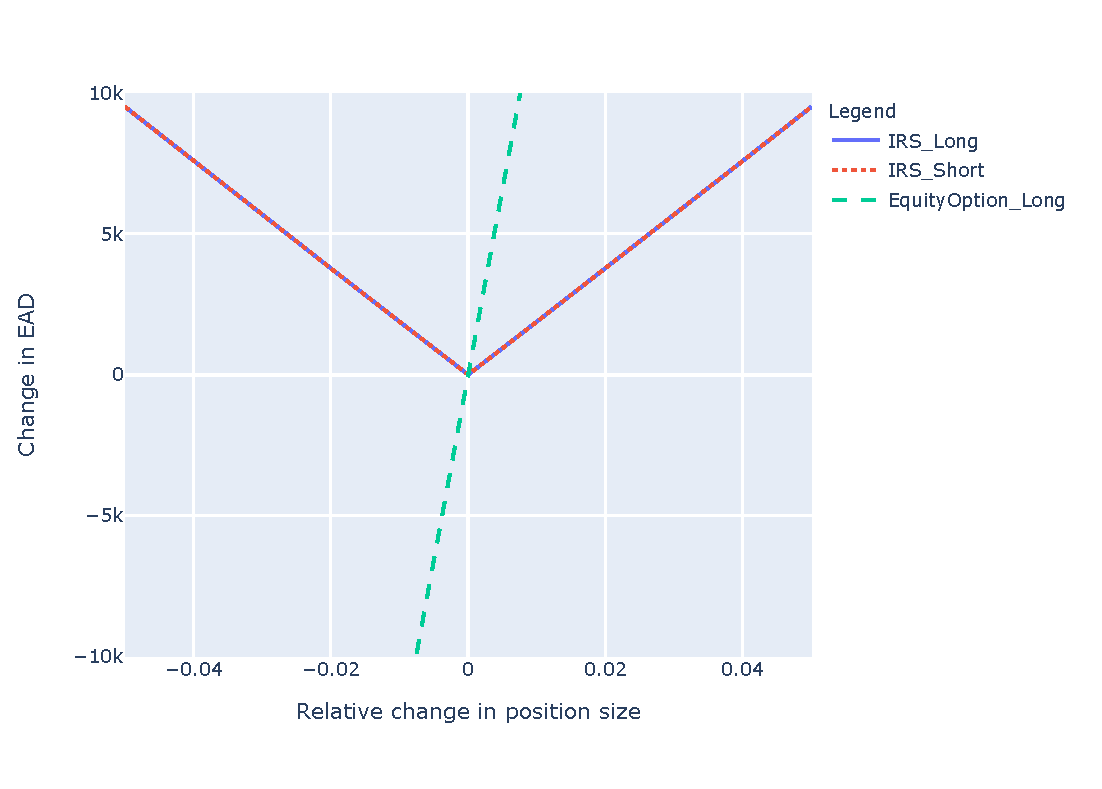
\includegraphics{Graphics/Indifferentiabililty_of_EAD.pdf}
        \caption[Non-differentiability of \gls{SA-CCR} \gls{EAD}]{When increasing or decreasing the notional of one of the two \gls{IRS} we can see that \gls{SA-CCR} \gls{EAD} is not differentiable with regard to trade notional due to the perfect hedge between the two \gls{IRS}.}
        \label{fig:indifferentiability of ead}
    \end{figure}

    \begin{figure}
        \centering
        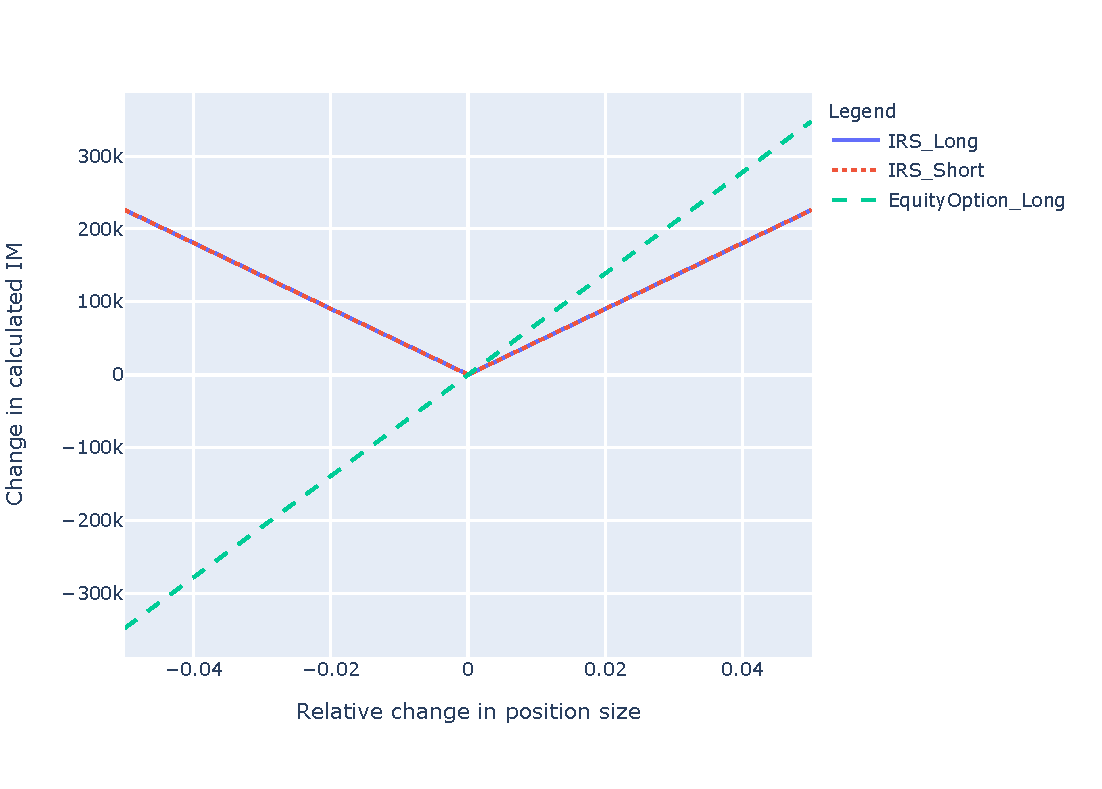
\includegraphics{Graphics/Indifferentiabililty_of_IM.pdf}
        \caption[Non-differentiability of \gls{ISDA SIMM}]{Same as figure \ref{fig:indifferentiability of ead} but for \gls{ISDA SIMM} initial margin}
        \label{fig:indifferentiability of im}
    \end{figure}
    
    \end{document}